\chapter{Robotic Operation of FACT}\label{chp:shifthelper}

From the very beginning, it was planned to operate \gls{fact} remotely,
to spare expenses and human resources,
since \gls{fact} is just a small experiment contributed to by four institutes.
For a few months after the first light in October 2011,
local operators steered the telescope from the container right next to the telescope.
Tasks were further automated and \gls{fact} could be operated fully remotely by July 2012~\cite{fact-design-operation}.
Further steps to minimize the amount of work the operators had to do were
made to the point were the telescope operated automatically,
without human interaction, after the startup each night.
Now, the operators only duty was to stay awake, monitoring the system and weather
conditions, only acting when something went wrong.
Error conditions include systems failure, wind or clouds coming up.
This developed to be a strenuous task, especially in nights with perfect conditions
operators were awake without ever needing to do anything.
So the question arose, if it was possible to implement a system allowing
the operators to sleep and only be alarmed if human interaction became necessary.
This system called the \texttt{shifthelper} was developed and tested in several iterations,
mainly by Dominik Neise and me.
After a lengthy period of tests, the \gls{fact} collaboration decided the system
was ready and operators could sleep at night at the end of 2017.

In this chapter, I will discuss the automatization and remote control infrastructure
of \gls{fact} and how the \texttt{shifthelper} was build on top of these
existing systems to enable robotic operation.

\section{Remote Control Infrastructure}
\begin{wrapfigure}[18]{O}{0.4\textwidth}
  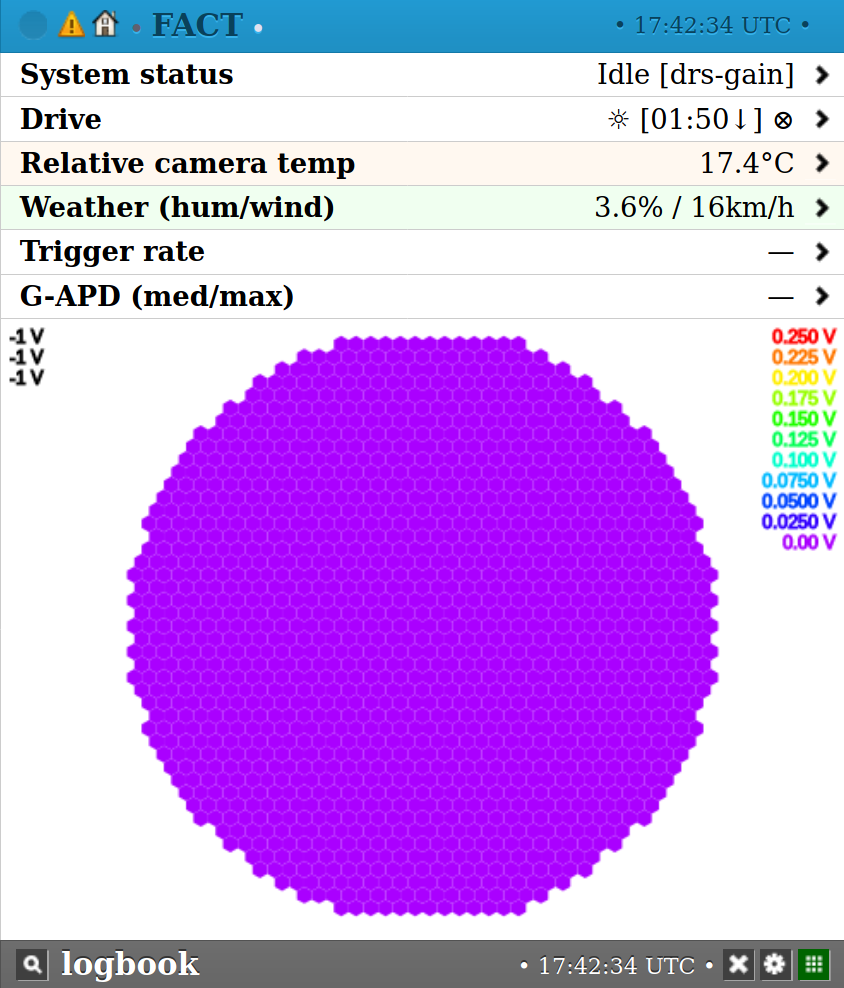
\includegraphics[width=\linewidth]{images/smartfact.png} 
  \caption{%
    Homepage of \texttt{SmartFact}, the webinterface for the remote operation of
    \gls{fact} during day time.
  }\label{fig:smartfact}
\end{wrapfigure}
\noindent \gls{fact} comprises many subsystems that need to work in unison for
observations.
The different subsystems provide information about the telescope's status,
weather conditions and most importantly steer the telescope, configure the 
telescope's hardware and take data.
The communication is performed over an inter-process communication
system based on the \gls{dim}~\cite{dim} library. 
Each subsystem is a \gls{dim} service, which can implement status updates
and/or commands.
\gls{dim}-clients can request status updates at regular intervals or on changes and can
issue commands.

The telescope's operation is steered using JavaScript and a webinterface
called \texttt{SmartFact} provides the current status of the telescope,
weather information, the possibility to manually control the
drive and the ability to start operation scripts.
A screenshot of the front page is shown in \autoref{fig:smartfact}.

The observation steering scripts are interpreted on the FACT web server
and write commands into the \gls{dim} network and receive status updates from it.
During the night, the script \texttt{Main.js} runs a loop getting 
the observation schedule from a database and executing the scheduled measurements
by sending the appropriate \gls{dim} commands.
Operators are assigned to observation nights using a calendar application and
while there is a webinterface for the observation schedule,
this is also filled automatically nowadays.
As an example, the schedule for December \nth{19}, 2019 is shown in \autoref{tab:schedule}.
This night, observations for five sources were carried out and the shift was
eleven and a half hours long.

Startup in the evening is organized via working through a checklist, 
which includes—among other things—inspecting the telescope via a live camera feed,
powering the drive electronics,
and starting execution of the \texttt{Main.js} script.

During the night, the system and weather conditions have to be monitored.
This was the task of the operator, who needed to stay awake for the whole preparation and observation time, which is over eleven hours in winter.

The most critical task is the shutdown of the telescope in the morning,
as the telescope is a serious fire hazard~\cite{hegra-fire},
if not in its parking position due North during daylight.
After the shutdown procedure is executed, the operator goes through a checklist
again and the result is stored in the \gls{fact} database.
Before the \texttt{shifthelper} was deployed, not filling this checklist only
resulted in an email to the \gls{fact} collaboration,
easily missed completely or seen to late to react in time.

\section{The \texttt{shifthelper}}
To move to fully automated data taking without a human operator
needed to keep an eye on system status and weather conditions,
the \texttt{shifthelper}\footnote{\url{https://github.com/fact-project/shifthelper}} has been developed.
As a continuously running service,
the \texttt{shifthelper} performs all checks previously done manually by the operators.
Additional checks were added to make sure the observations are started in the 
evening, the telescope is parked in the morning,
possible alerts have indeed reached a human operator,
and the \texttt{shifthelper} itself is running.

\begin{wraptable}[11]{O}{0.4\textwidth}
  \caption{Schedule for 2019-12-19.}
  \label{tab:schedule}%
  \tablefont%
  \begin{tabular}{l l l}
    \toprule
    Time & Type & Source \\
    \midrule
    19:03 & Startup & — \\
    19:18 & Data & 1ES 1959+650 \\
    21:22 & Data & 1ES 2344+51.4 \\
    00:35 & Data & Crab \\
    04:03 & Data & PKS 0736+01 \\
    05:21 & Data & Mrk 421 \\
    06:22 & Shutdown & — \\
    \bottomrule
  \end{tabular}
\end{wraptable}

In the following, three central concepts of the \texttt{shifthelper} will be introduced:
checks, messages and notifiers.
A check is a task running regularly, e.\,g.\ every minute or at certain
times, which can emit messages with different categories and severity levels that
are pushed into a common message queue.
Notifiers relay messages pushed into the queue to recipients.
A number of notifiers have been implemented in the \texttt{custos}~\cite{custos} library that
was developed for the \texttt{shifthelper}.
Messages can be send via email, as instant messages using Telegram~\cite{telegram},
by phone calls using the provider Twilio~\cite{twilio},
by issuing http post requests to a web page or just logging messages to file or console.
The \texttt{shifthelper} makes use of the instant messages, phone calls, website and logging facilities.
The severity level is represented as an integer, comparable to common logging libraries. 
Notifiers have a level setting under which messages will not be relayed to the
recipients and messages can be relayed to different recipients depending on the category of a message.
This is used in the \texttt{shifthelper} to call either the current operator for problems
directly related to the observations or an expert in case of 
problems with the \texttt{shifthelper} itself or if no operator is available.
For notifiers that support it, e.\,g.\ email and Telegram, files and images can be attached.

\begin{figure}
  \centering
  \begin{tikzpicture}
  \tikzset{
  lapalma/.style={draw=darkRed, thick, rounded corners},
  dortmund/.style={draw=tugreen, thick, rounded corners},
  external/.style={draw=darkBlue, thick, rounded corners},
}

\node[lapalma, font=\large\ttfamily, anchor=east, align=center] (smartfact) at (0, 0) {\strut smartfact};
\node[lapalma, anchor=east, align=center] (database) at (0, -1.5) {%
  
\includegraphics[width=1.5cm]{images/mysql.pdf} 
};
\node[lapalma, font=\large\ttfamily, anchor=east, align=center] (heartbeat) at (0, 1.5) {\strut heartbeat};


\node[dortmund, font=\large\ttfamily, anchor=center, align=center] (shifthelper) at (3, 0) {\strut shifthelper};

\node[dortmund, font=\large\ttfamily, anchor=west, align=center] (webinterface) at (6, 2) {\strut webinterface};

\node[external, anchor=center, align=center, anchor=west] (telegram) at (6, 0) {%
  
\includegraphics[height=1cm]{images/telegram.png}\\
  Messenger%
};
\node[external, anchor=center, align=center, anchor=west] (twilio) at (6, -2.2) {%
  
\includegraphics[width=2cm]{images/twilio.png}\\
  Call Provider%
};

\tikzset{>={Stealth[length=3mm]}}
\draw[thick, black, <-] (shifthelper.west) to [out=150, in=0] (smartfact.east);
\draw[thick, black, <-] (shifthelper.west) to [out=230, in=0] (database.east);

\draw[thick, black, ->] (shifthelper.east) to[out=0, in=180] (telegram.west);
\draw[thick, black, <->] (shifthelper.east) to[out=30, in=220] (webinterface.west);
\draw[thick, black, ->] (shifthelper.east) to[out=-70, in=180] (twilio.west);

\draw[thick, black, <->] (heartbeat.east) to[out=0, in=160] (webinterface.west);

\node[anchor=west, align=center, font=\large, right=0.5cm of telegram.east]  {%
  {\fontsize{60}{60}\faBed \selectfont}\\
  Shifter-On-Call%
};

  \end{tikzpicture}
  \caption{%
    Structure of the \texttt{shifthelper} infrastructure.
    The services in red are running on the computers in the counting container on
    La Palma, the ones in green are running on a server at TU Dortmund and
    the blue ones are external services.
    The arrows show the flow directions of information.
  }\label{fig:shifthelper}
\end{figure}

\begin{table}
  \centering
  \caption{%
    Checks performed by the \texttt{shifthelper}.
    Most checks are only performed during scheduled data taking,
    between 10 minutes before the scheduled startup and the shutdown task.
    Only the check if the operator performed the shutdown is done after the scheduled
    shutdown time.
  }\label{tab:checks}
  \begin{tabular}{p{0.8\textwidth} l}
    \toprule
    Condition & Callee \\
    \midrule
    Is the \texttt{SmartFact} website up to date? & Operator \\
    Is weather information available? & Operator \\
    Is an operator in the calendar for the night? & Expert \\
    Is \texttt{Main.js} running? & Operator \\
    Is the wind speed slower than \SI{50}{\km\per\hour} if the telescope is not parked & Operator \\ 
    Is the wind gust speed slower than \SI{50}{\km\per\hour} if the telescope is not parked & Operator \\ 
    Is the median camera current less than \SI{115}{\micro\ampere} & Operator \\ 
    Is the maximum camera current less than \SI{160}{\micro\ampere} & Operator \\ 
    Is the camera cooling working? & Operator \\
    Low trigger rate for longer than ten minutes? & Operator \\
    Is the temperatures of the container nominal?  & Operator \\
    Is the operator awake 20 minutes before shutdown? & Operator \\
    Is the parking checklist filled after shutdown? & Operator \\
    Is the \texttt{heartbeat} program running? & Expert \\
    Two checks if the \gls{dim} network is operating correctly & Operator \\
    Three different checks for correct operation of the bias voltage supply & Operator \\
    A dummy alert, can be triggered by the operator to test the configuration & Operator \\
    \bottomrule
  \end{tabular}
\end{table}

The \texttt{shifthelper} is running  on a server in continental Europe, either in Dortmund
or at ETH Zurich,
so that it can still alert the operator even if power was lost at the telescope site
or internet access at the observatory is not possible.
The current operator is queried from the FACT database running at the observatory,
while a fallback operator and the expert are set for longer periods in a configuration file to also work
in case no internet connection to La Palma is possible.
To be safe for short losses of connection, the parts of the database needed 
by the \texttt{shifthelper} are cached on the server the \texttt{shifthelper} is running on and
synced with the database on La Palma every minute.


The checks currently performed by the \texttt{shifthelper} are listed in \autoref{tab:checks}
together with who is called in case the check fails.
Most of these checks are only performed during planned observations,
defined as ten minutes before the scheduled startup and the scheduled shutdown.
A lower level of checks makes sure the information provided through \texttt{SmartFact} 
is up to date, e.\,g.\ \texttt{SmartFact} is running and weather information has been updated in the last ten minutes.
Checks monitoring the environmental conditions are using two weather stations
on the Roque not far from \gls{fact}, provided by \gls{magic} and the Telescopio Nazionale Galileo, the data is exposed through \texttt{SmartFact}.
Currently, only wind speed is monitored as rain is considered not harmful for the telescope.
During observations with strong moonlight, it can happen that the \gls{sipm} current
exceeds safety limits.
Two limits are defined and checked by the \texttt{shifthelper}, one for the median current
over all pixels and one for the maximum camera current.
During the night, it is checked if a script is running, so that when \texttt{Main.js} exits
due to an error or was never started in the beginning of the night, the operator is notified.
Several checks monitor the state of different subsystems of \gls{fact},
including the bias voltage supply for the pixels.
Most importantly, it is checked if the human operator is awake to supervise the shutdown 
procedure and that the shutdown checklist has been filled.

Exceptions occurring while the shifthelper performs its checks result in a message
to the expert, notifying him or her of the error condition.
Through this very general instrument, the \texttt{shifthelper} identified several unanticipated error conditions and immediately notified the collaboration.
This includes network outages on La Palma, power losses in the observatory and a hardware failure.


Since first testing began in 2016, costs for phone calls have cumulated at around 
350 €.
Operators should normally not answer the phone calls to reduce costs,
and most calls are indeed free of charge.
Large parts of the costs were generated by few operators sending calls to their mailboxes,
something now easily avoided by making operators aware of the issue.
Compared to the cost of human labor, this is a rather small amount of money for 
nearly four years of operation\footnote{\gls{fact} operators were not paid directly 
for the night shifts. Rather it was expected of collaboration members to perform these
shifts. However, the night shifts took a toll on the operators and usually reduced 
the ability to work on their day job, e.\,g.\ as research assistant}.



\section{Webinterface}
To display the current alerts and to make sure the operator has received and acknowledged a message, a web service has been developed.
It receives messages from the \texttt{shifthelper} via http \texttt{POST} requests and
displays a list of alerts.
Operators have to acknowledge the alerts by pressing a button.
If an alert is not acknowledged within 15 minutes,
the fallback operator is called to take over.
Acknowledging an alert will also prevent the \texttt{shifthelper} for calling the operator
for the same reason for a time period of ten minutes, giving the operator time
to check what has happened and probably solving the issue.
A screenshot of the webinterface is shown in \autoref{fig:webinterface}.
The webinterface uses the WebSocket protocol to push new alerts to the connected
clients, so they directly appear without refreshing the page.

The webinterface is also used to check if the human operator is awake twenty minutes
before the scheduled shutdown.
For this, the operator has to push a button on the webinterface.

\begin{figure}
  \begin{captionbeside}{%
    Screenshot of the \texttt{shifthelper} homepage, showing the most recently received
    heartbeats and the list of alerts.
    The dummy alert is part of the startup checklist and is issued by the
    operator via the webinterface to make sure the \texttt{shifthelper} is running and  has the correct contact
    information.
    The webinterface is optimized for use on small screens such as mobile phones.
    \label{fig:webinterface}%
  }%
    \raisebox{\dimexpr\baselineskip-\totalheight\relax}{%
      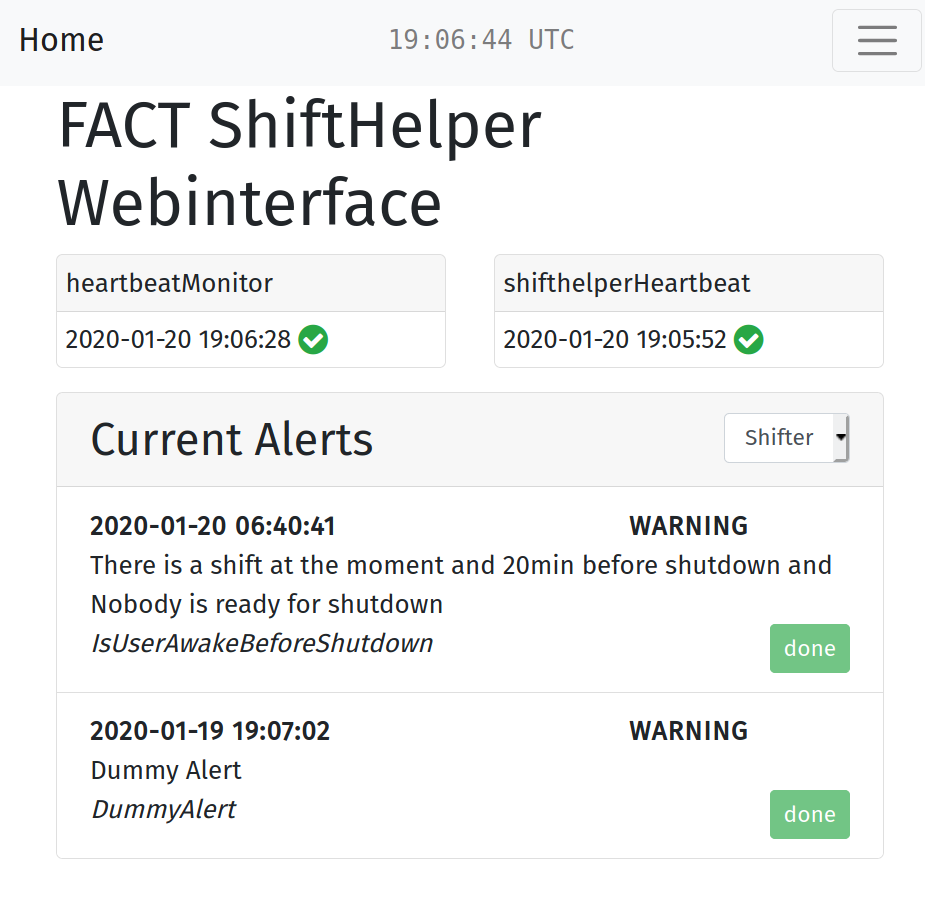
\includegraphics[width=0.5\textwidth]{images/shifthelper_webpage.png}%
    }%
  \end{captionbeside}
\end{figure}

\section{Heartbeat}

To make sure the \texttt{shifthelper} is up and running,
it posts a heartbeat timestamp every minute to the webinterface which is checked
by a program running on La Palma.
In case the timestamp is not available or older than 10 minutes, 
the heartbeat program calls the expert. 
In turn, the heartbeat program also posts a timestamp to the webinterface which
is checked by the \texttt{shifthelper} itself, thus providing strong guarantees
that both programs are running at all times minimizing the chances of unnoticed failure. 
